\documentclass[letterpaper]{article}
\usepackage{underscore}
\usepackage[left=2.0cm, right=2.0cm, top=2.0cm]{geometry}
\usepackage[utf8]{inputenc}
\usepackage{graphicx}
\usepackage{graphics}
\usepackage[spanish]{babel}
\usepackage{lipsum}
\usepackage{float}
\usepackage{subfigure}

\usepackage{color}

\title{EV\_2\_4\_giro\_de\_un\_motor\_de\_corriente\_directa}
\author{Ledesma Hernández Miguel Ángel}

\begin{document}

\maketitle
\vspace{10cm}
\begin{center}
4-A Mecatrónica\\
Electrónica de potencia \\
\end{center}


\vspace{3cm}
\begin{center}
Universidad politécnica de la zona metropolitana de Guadalajara\\
\end{center}





\newpage

\begin{large}
Para comenzar a entender ¿cómo es que gira un motor de corriente directa? debemos entender de primeras cómo es que funciona un motor y que es un motor de corriente directa.\\De esta manera podremos saber cómo es que debemos hacer para invertir la rotación de un motor\\
Un motor de corriente continua tambien se le puede llamar motor de corriente directa, motor DC, motor CC debido a sus iniciales "Directly current", El motor es un elemento que transforma la energía electrica en energía mecánica al pasar por un proceso de energía electromágnetica.
El motor tiene una parte fija que es el estator. Esta provee de un campo magnetico, tiene un rotór que es la parte que gira es simplemente una espira o dependiendo un conjunto de espiras al que llamamos arrojamiento o bobina, cada motor tiene un colector y cada vez que circula una corriente por el anillo se porduce una delg, en cuanto sucede esto cumple con la ley de Lawrence, aplicando esto y en que sentido va la corriente del campo, se cumplen las condiciones para la ley de Lawrence, y este será el sentido de nuestro motor. como podemos ver en la siguiente imagen\\

\end{large}
\begin{figure}[hbtp]
\caption{Motor}
\centering
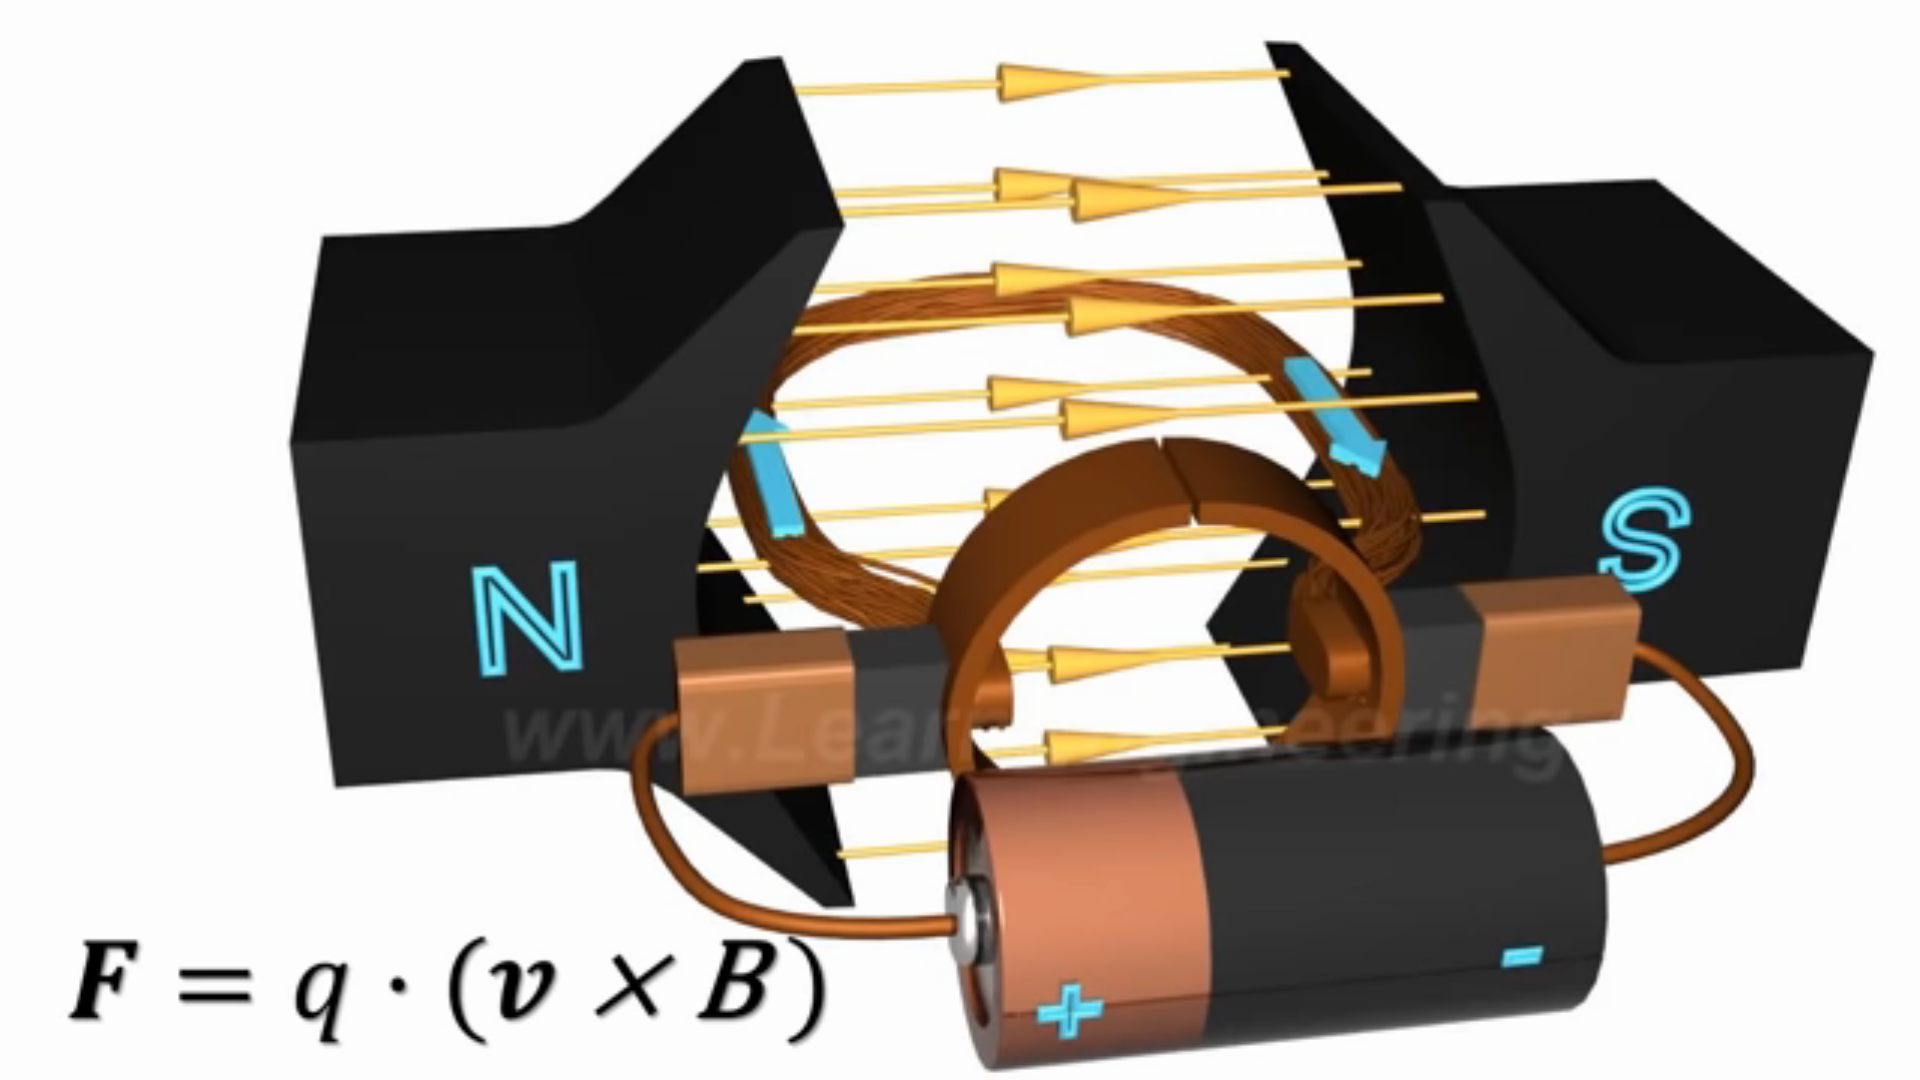
\includegraphics[scale=.2]{motore.png}
\end{figure}
\begin{large}
Ahora que sabemos que es y como funciona un motor debemos saber como girar un motor en ambos sentidos; Para ello de la manera mas simple será tomando la corriente e invirtiendola, de esta manera el campo mágnetico irá en orden inverso a como estaba originalmente y la rotación será contraria, para ello podemos usar un switch de polaridad, como el de la siguiente imagen\\
\end{large}
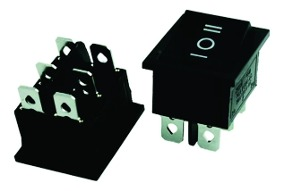
\includegraphics[scale=1]{chuicheinversor.jpg} 
\begin{large}
Tambien son usados los puentes H, que en si dice, no pase corriente por una parte, pasa por la otra y como los mosfet o algunos puentes H tienen diodos impiden el paso de corriente dando cabida al otro lado del circuito que hará que circule de manera inversa, pasando por el moto, como se ve en la sig imagen.\\
\end{large}
\begin{figure}[hbtp]
\caption{Puente H}
\centering
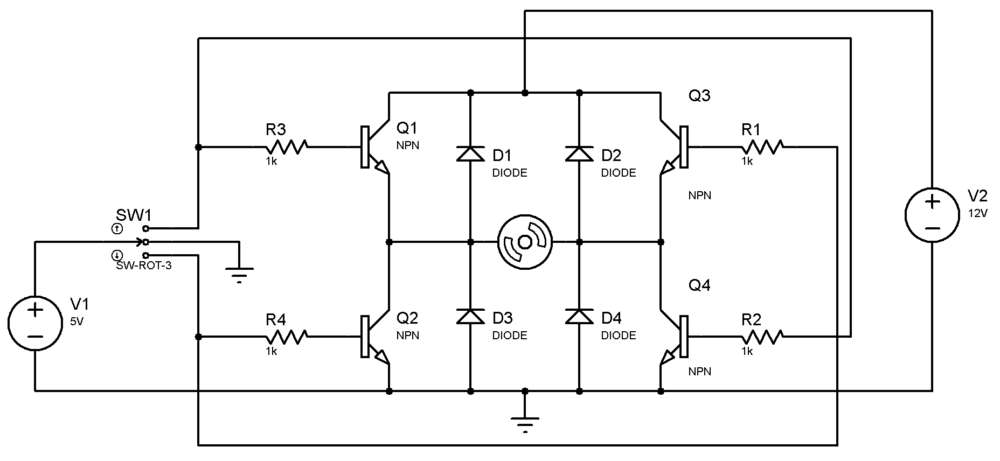
\includegraphics[scale=1.3]{puenteashe.png}\\
\end{figure}

\begin{huge}
Bibliografias\\
\end{huge}
@Book{ 9788428399012,
  title     = {Motores de corriente continua},
  publisher = {Ediciones Paraninfo, S.A},
  year      = {2014},
  author    = {José Roldán},
  isbn      = {9788428399012},

}

\end{document}